
\begin{table}[!ht]
\centering
\resizebox{\columnwidth}{!}{\begin{tabular}{|c|c|c|c|} 
\hline
item & Machine hours & Craftman's hours & profit \\
\hline
Tennis Racket & 1.5 & 3  &  20  \\ 
\hline
Cricket Bats & 3 & 1 &  10  \\ 
\hline
Maximum time Available & 42 & 24 & \\ 
\hline
\end{tabular}}
\caption{factory Requirements}
\label{opt/14/tab:table1}
\end{table}
Let the number of Tennis Rackets  be $x$ and the number of cricket bats be $y$  such that 
\begin{align}
x \geq 0 \\
y \geq 0 
\end{align}
According to the question,
\begin{align}
1.5x+3y &\leq 42 \\
\implies 3x+6y &\leq 84 \\
\implies x+2y &\leq 28 
\end{align}
and,
\begin{align}
3x+y &\leq 24 
\end{align}
$\therefore$ Our problem is
\begin{align}
\max_{\vec{x}} Z &= \myvec{20 & 10}\vec{x}\\
s.t. \quad \myvec{1 & 2 \\ 3 & 1}\vec{x} &\preceq \myvec{28\\24} 
\end{align}
Lagrangian function is given by
\begin{equation}
\begin{aligned}
&L(\vec{x},\boldsymbol{\lambda}) \\ &= \myvec{20 & 10}\vec{x}+\lcbrak{\sbrak{\myvec{1 & 2}\vec{x}-28}} \\ &+ \sbrak{\myvec{3 & 1}\vec{x}-24}\\ &+ \sbrak{\myvec{-1 & 0}\vec{x}} +\rcbrak{\sbrak{\myvec{0 & -1}\vec{x}}}\boldsymbol{\lambda}
\end{aligned}
\end{equation}
where,
\begin{align}
\boldsymbol{\lambda} &= \myvec{\lambda_1 \\ \lambda_2 \\ \lambda_3 \\ \lambda_4 \\ \lambda_5 \\ \lambda_6}
\end{align}
Now,
\begin{align}
\nabla L(\vec{x},\boldsymbol{\lambda}) &= \myvec{20+ \myvec{1 & 3  & -1 & 0 }\boldsymbol{\lambda}\\ 10+\myvec{2 & 1 & 0 & -1}\boldsymbol{\lambda} \\ \myvec{1 & 2}\vec{x}-28 \\ \myvec{3 & 1}\vec{x}-24 \\  \myvec{-1 & 0}\vec{x} \\ \myvec{0 & -1}\vec{x}}
\end{align}
$\therefore$ Lagrangian matrix is given by
\begin{align}
\myvec{0 & 0 & 1 & 3 & -1 & 0 \\ 0 & 0 & 2 & 1  & 0 & -1 \\ 1 & 2 & 0 & 0 & 0 & 0 \\ 3 & 1 & 0 & 0 & 0 & 0  \\ -1 & 0 & 0 & 0 & 0 & 0  \\ 0 & -1 & 0 & 0 & 0 & 0 }\myvec{\vec{x} \\ \boldsymbol{\lambda} } &= \myvec{-20 \\ -10 \\ 28 \\ 24 \\ 0 \\0 }
\end{align}
Considering $\lambda_1,\lambda_2$ as only active multiplier,
\begin{align}
\myvec{0 & 0 & 1 & 3 \\ 0 & 0 & 2 & 1 \\ 1 & 2 & 0 & 0 \\ 3 & 1 & 0 & 0}\myvec{\vec{x}\\ \boldsymbol{\lambda}} &= \myvec{-20 \\ -10 \\ 28 \\ 24}
\end{align}
resulting in,
\begin{align}
\myvec{\vec{x} \\ \boldsymbol{\lambda}} &= \myvec{0 & 0 & 1 & 3 \\ 0 & 0 & 2 & 1 \\ 1 & 2 & 0 & 0 \\ 3 & 1 & 0 & 0}^{-1}\myvec{-20 \\ -10 \\ 28 \\ 24}
\\
\implies   \myvec{\vec{x} \\ \boldsymbol{\lambda}} &= \myvec{0 & 0 & \frac{-1}{5} & \frac{2}{5} \\ 0 & 0 & \frac{3}{5} & \frac{-1}{5} \\ \frac{-1}{5} & \frac{3}{5} & 0 & 0 \\ \frac{2}{5} & \frac{-1}{5} & 0 & 0}\myvec{-20 \\ -10 \\ 28 \\ 24}
\\
\implies \myvec{\vec{x} \\ \boldsymbol{\lambda}} &= \myvec{4 \\ 12 \\ -2 \\ -6 }
\end{align}
$\because \boldsymbol{\lambda}=\myvec{-2 \\ -6} \succ \vec{0} $
\\
$\therefore$ Optimal solution is given by
\begin{align}
\vec{x} &= \myvec{4\\12} \\
Z &= \myvec{20 & 10}\vec{x} \\
&= \myvec{20 & 10}\myvec{4 \\ 12} \\
&= 200
\end{align}
By using cvxpy in python ,
\begin{align}
\vec{x}=\myvec{3.99999998\\12.0000000}\\
Z = 199.99999964
\end{align}
Hence ,\boxed{x=4} Tennis Rackets and \boxed{y=12} Cricket Bats should be used to maximum time Available profit \boxed{Z=200} as can be
verified from Fig. \ref{opt/14/fig: Graphical Solution}.	
\begin{enumerate}
\item 4 Tennis Rackets and 12 Cricket Bats must be made so that factory runs at full capacity.
\item Maximum profit is Rs 200, When 4 Tennis Bats and 12 Cricket Bats are produced.
\end{enumerate}
%
\begin{figure}[!ht]
\centering
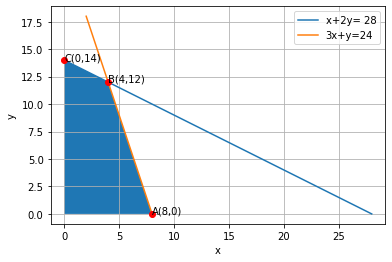
\includegraphics[width=\columnwidth]{solutions/su2021/2/14/download.png}
\caption{Graphical Solution}
\label{opt/14/fig: Graphical Solution}	
\end{figure}

